% Подписи колонтитула
\newcommand{\colontitulAutors}{astronom\_v\_cube, edombek et al.}
\newcommand{\colontitulYear}{2022}
\newcommand{\colontitulEducationalSubject}{Алгоритмы решения задач по теории колебаний}
\newcommand{\colontitulTeacher}{Сутягин А.А.}

%Настройки шаблона
\documentclass[10pt,landscape,a4paper]{article}
\usepackage[utf8]{inputenc}
\usepackage[english, russian]{babel}
\usepackage[T1,T2A]{fontenc}  
\usepackage{upgreek} % прямые греческие ради русской традиции
\usepackage{tikz}
\usetikzlibrary{shapes,positioning,arrows,fit,calc,graphs,graphs.standard}
%\usepackage[nosf]{kpfonts}
%\usepackage[t1]{sourcesanspro}
\usepackage{multicol}
\usepackage{wrapfig}
\usepackage[top=6mm,bottom=8mm,left=4mm,right=4mm]{geometry}
\usepackage[framemethod=tikz]{mdframed}
\usepackage{microtype}
\usepackage{pdfpages}
\usepackage{amsthm,amsmath,amscd}   % Математические дополнения от AMS
\usepackage{amsfonts,amssymb}       % Математические дополнения от AMS
\usepackage{mathtools}              % Добавляет окружение multlined
\usepackage{xfrac}                  % Красивые дроби
\usepackage{physics}

\usepackage{fancyhdr} % колонтитулы

%некоторые математические команды
\newcommand{\Div}{\operatorname{div}}
\newcommand{\Grad}{\operatorname{grad}}

\let\bar\overline

\definecolor{myblue}{cmyk}{1,.72,0,.38}

\def\firstcircle{(0,0) circle (1.5cm)}
\def\secondcircle{(0:2cm) circle (1.5cm)}

\colorlet{circle edge}{myblue}
\colorlet{circle area}{myblue!5}

\tikzset{filled/.style={fill=circle area, draw=circle edge, thick},
	outline/.style={draw=circle edge, thick}}

\pgfdeclarelayer{background}
\pgfsetlayers{background,main}

%\everymath\expandafter{\the\everymath \color{myblue}}
\everydisplay\expandafter{\the\everydisplay \color{myblue}}

\renewcommand{\baselinestretch}{.8}
\pagestyle{empty}

\global\mdfdefinestyle{header}{%
	linecolor=gray,linewidth=1pt,%
	leftmargin=0mm,rightmargin=0mm,skipbelow=0mm,skipabove=0mm,
}

\makeatletter % Author: ttps://tex.stackexchange.com/questions/218587/how-to-set-one-header-for-each-page-using-multicols
\renewcommand{\section}{\@startsection{section}{1}{0mm}%
	{.2ex}%
	{.2ex}%x
	{\color{myblue}\sffamily\small\bfseries}}
\renewcommand{\subsection}{\@startsection{subsection}{1}{0mm}%
	{.2ex}%
	{.2ex}%x
	{\sffamily\bfseries}}

\makeatother
\setlength{\parindent}{0pt}

%колонтитулы
\pagestyle{fancy}
\fancyhf{}
\setlength{\headheight}{40pt}
\setlength{\headsep}{4pt}
\renewcommand{\headrulewidth}{1pt}
\fancyhead[L]{\textcopyright~\colontitulAutors}
\fancyhead[C]{Программа минимум по курсу <<\colontitulEducationalSubject>> \colontitulYear г}
\fancyhead[R]{Преподаватель:~\colontitulTeacher}

\begin{document}
	\small
	\begin{multicols*}{2}

		\section{Гармонический осциллятор}

		\textit{Задачи, обычно, выглядят так: "Построить фазовый портрет и описать возможные колебательные режимы системы: $ \ddot{x} + f(x) = 0$"}\\
		\textbf{Построение фазового портрета:}\\
		Сначала составляем систему, принимая $\dot{x} = y$:\\
		$\begin{cases}
			\dot{x} = y \\
			\dot{y} = -f(x)
		\end{cases} $\\
		Приравниваем $\dot{y} = 0$, чтобы, решив уравнение, найти количество состояний равновесия и их координаты по $x$.\\
		Затем рассчитываем $U(x) = -\int f(x) \,dx $ - взятую с обратным знаком работу действующих в системе сил, или же - потенциальную энергию системы. Подставляя полученные выше состояния равновесия, находим значения энергии в состояниях равновесия, т.е. их координаты по $y$. Для получившегося выражения энергии строится график $U(x)$, а затем, снося различные уровни энергии, под ним строится фазовый портрет $\dot{x}(x)$.\\
		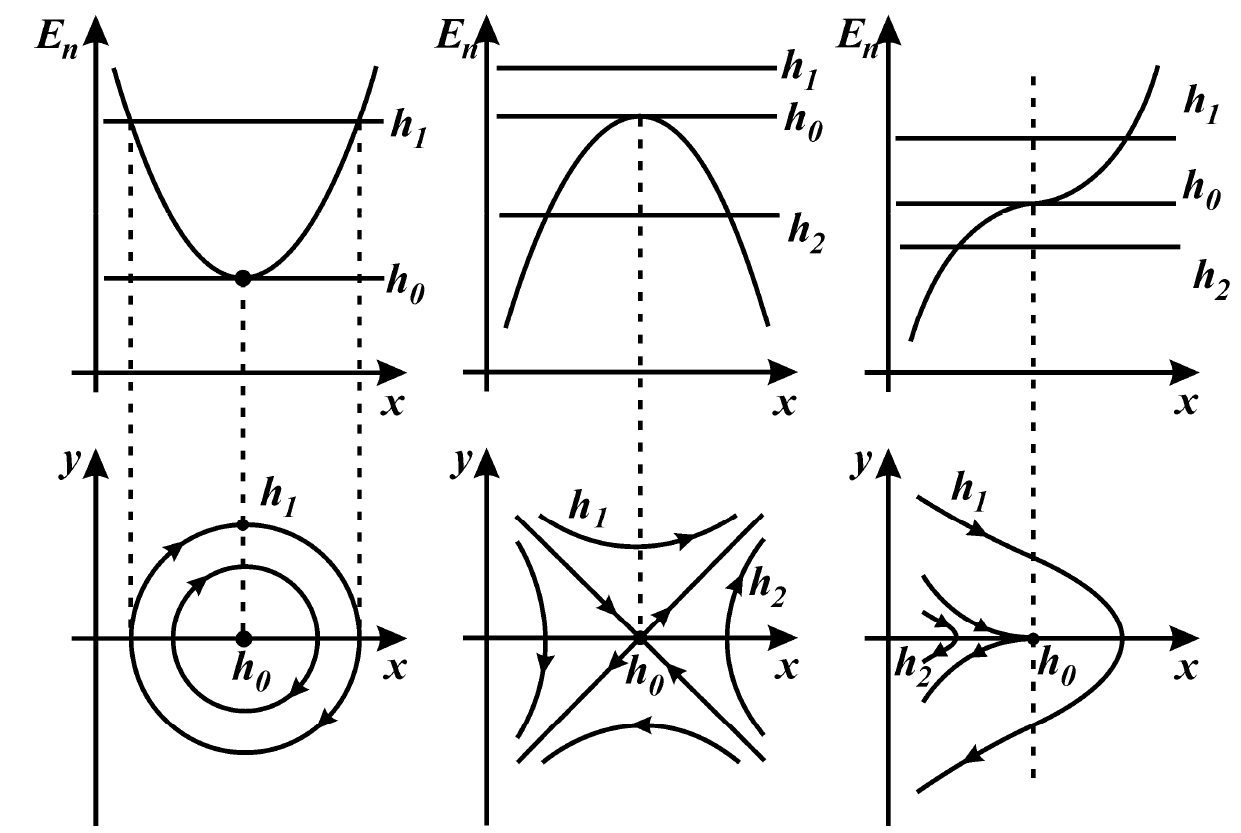
\includegraphics[width=0.5\linewidth]{tk_practice_img/oscill}
		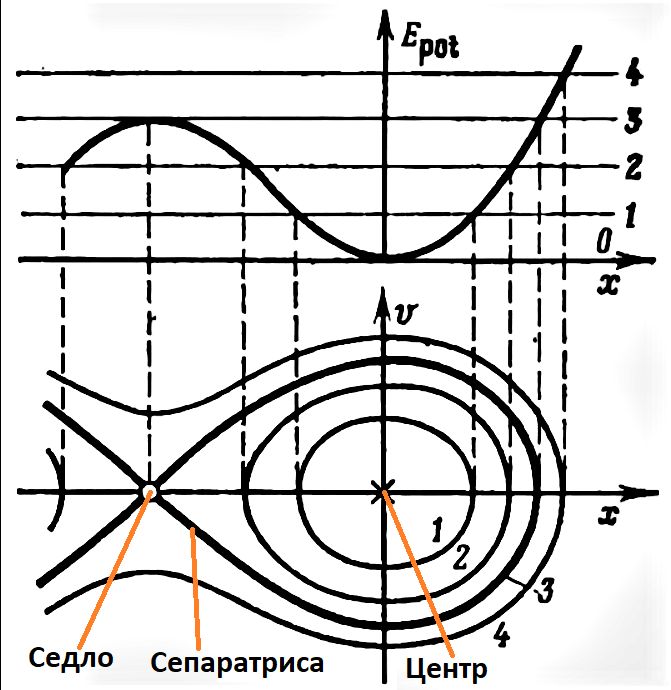
\includegraphics[width=0.35\linewidth]{tk_practice_img/oscill_2}\\
		\textbf{Анализ колебательных режимов:}\\
		не ебу\\

		\section{Задачи на системы быстрых и медленных движений}
		\textit{Задачи, обычно, выглядят так: "Исследовать динамику системы"} или \textit{"Построить разбиение фазовой плоскости на фазовые траектории для системы, описываемой уравнениями":\\
		$\begin{cases}
			\mu\dot{x} = f(x, y)\\
			\dot{y} = f(x)
		\end{cases}$}\\
		В задаче должен быть задан параметр $\mu$. В отличие от задач на Ван-Дер-Поля, должно быть ограничение значения параметра, например $0 < \mu \leqslant 1$.\\
		Задача заключается в построении систем медленных и быстрых движений, поиске состояний равновесия, построении фазового портрета и поиска возможного предельного цикла.  \\
		От расположения параметра $\mu$ в системе уравнений (либо около $x$, либо около $y$) зависит направление прямых на фазовом портрете. Если параметр расположен около $x$ – прямые горизонтальные, если около $y$ – вертикальные.\\ 
		По уравнению системы с параметром определяется направление стрелок путем подстановки различных точек выше и ниже фазовой траектории. Направление стрелок на самой же фазовой траектории определяется ???????. Система медленных движений определяет сам вид основной траектории и используется для нахождения состояний равновесия.\\ 
		\textbf{Составление системы БД:}\\
		1. Делим уравнение с параметром на сам параметр – получаем 1-е уравнение\\
		2. Делим одно уравнение исходной системы на второе и выявляем, что в данном случае является константой (например $x = x_0 = const$) – получаем 2-е уравнение.\\
		\textbf{Составление системы МД:}\\
		1. Первое уравнение остается неизменным\\
		2. Кладём параметр $\mu = 0$ – получаем 2-е уравнение. Затем, решая уравнение, находим точки пересечения с осью, после берём производную от полученного выше выражения, кладём её равной 0 и находим состояния равновесия.\\
		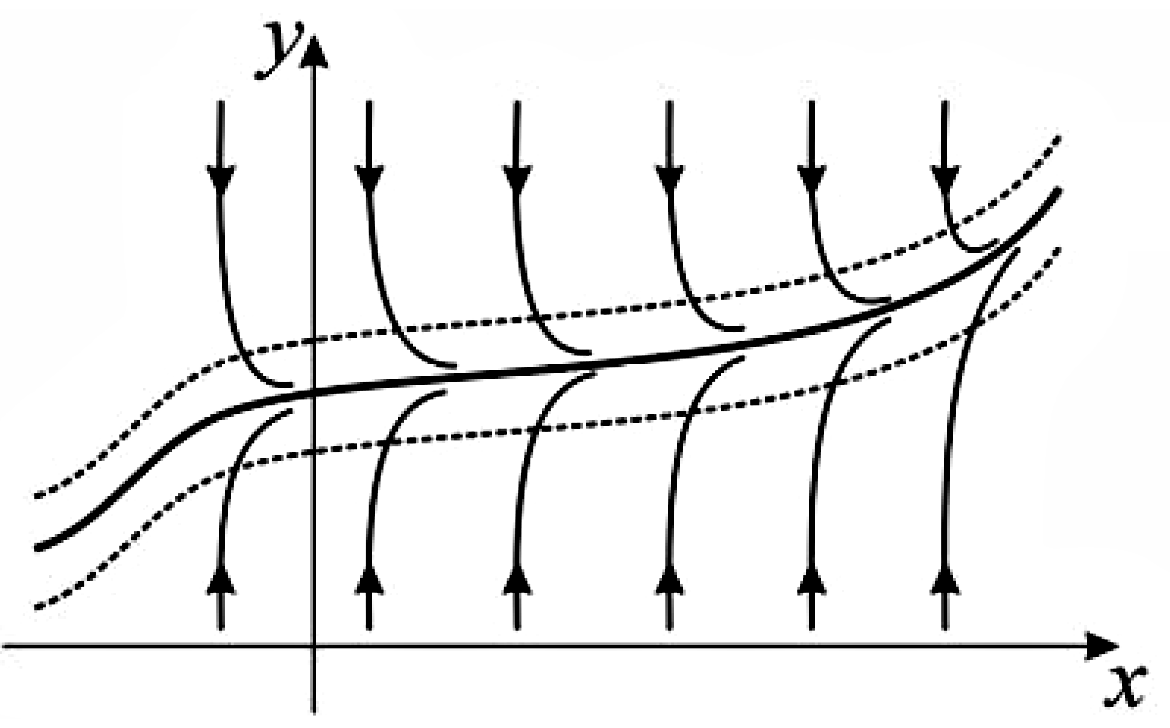
\includegraphics[width=0.5\linewidth]{tk_practice_img/sbmd_2}
		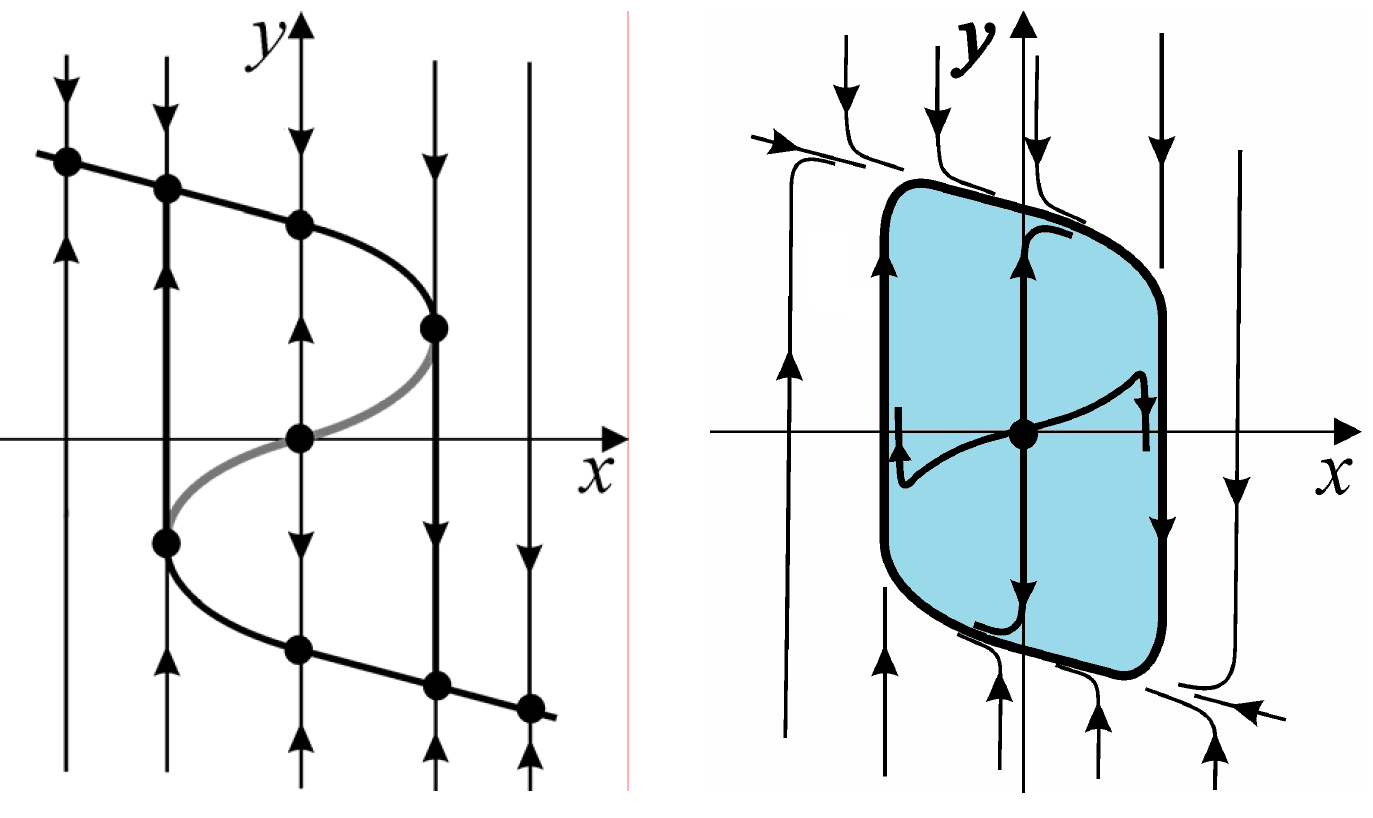
\includegraphics[width=0.5\linewidth]{tk_practice_img/sbmd}
		
		\section{Классификация состояний равновесия}
		
		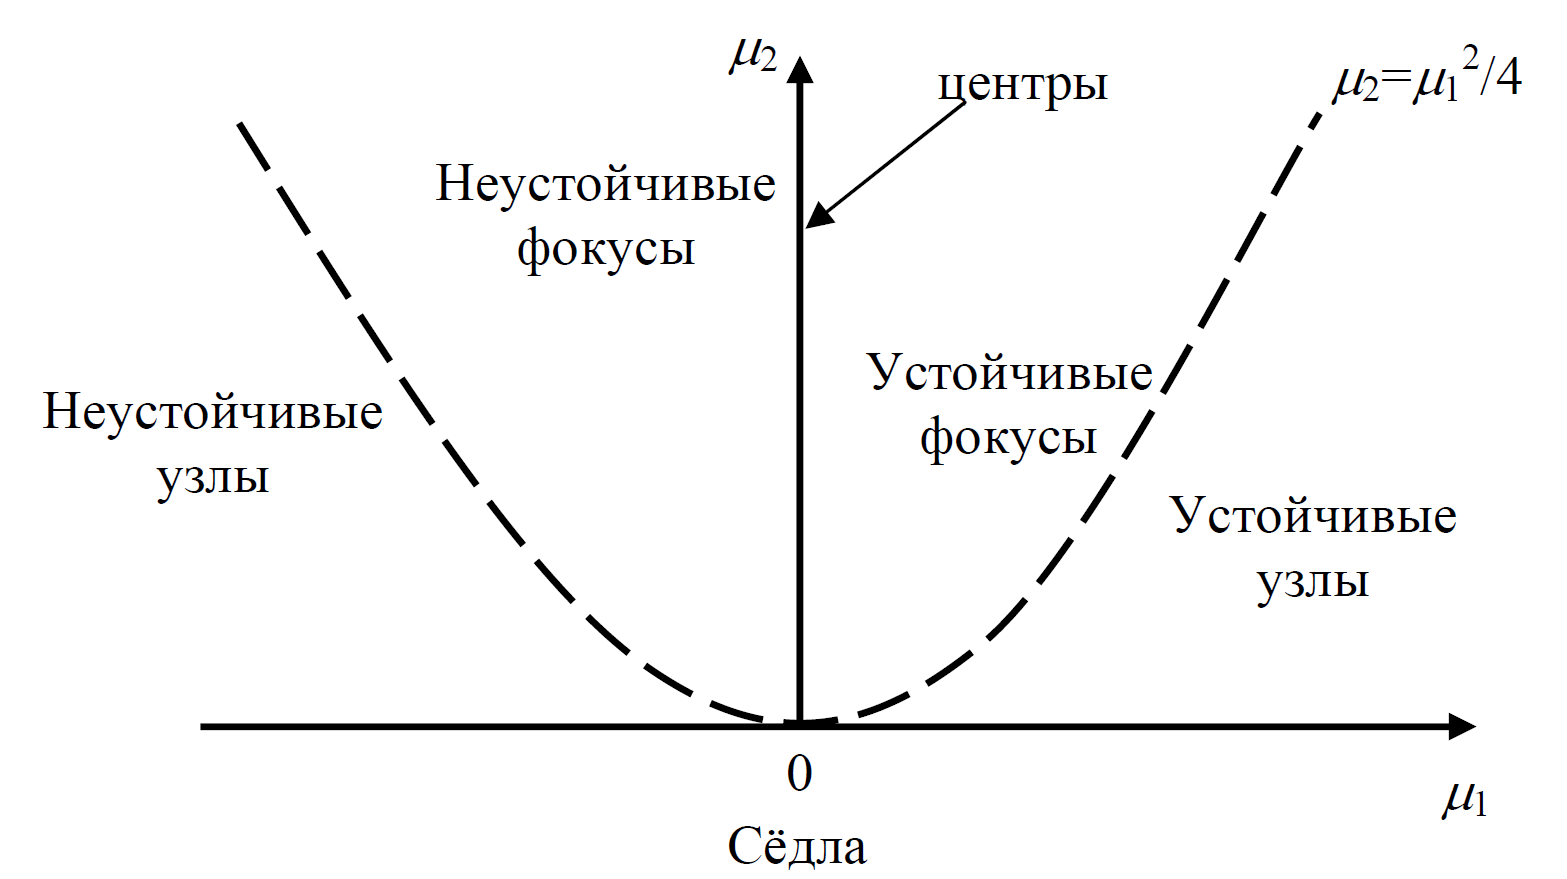
\includegraphics[width=0.5\linewidth]{tk_practice_img/classific_0}
		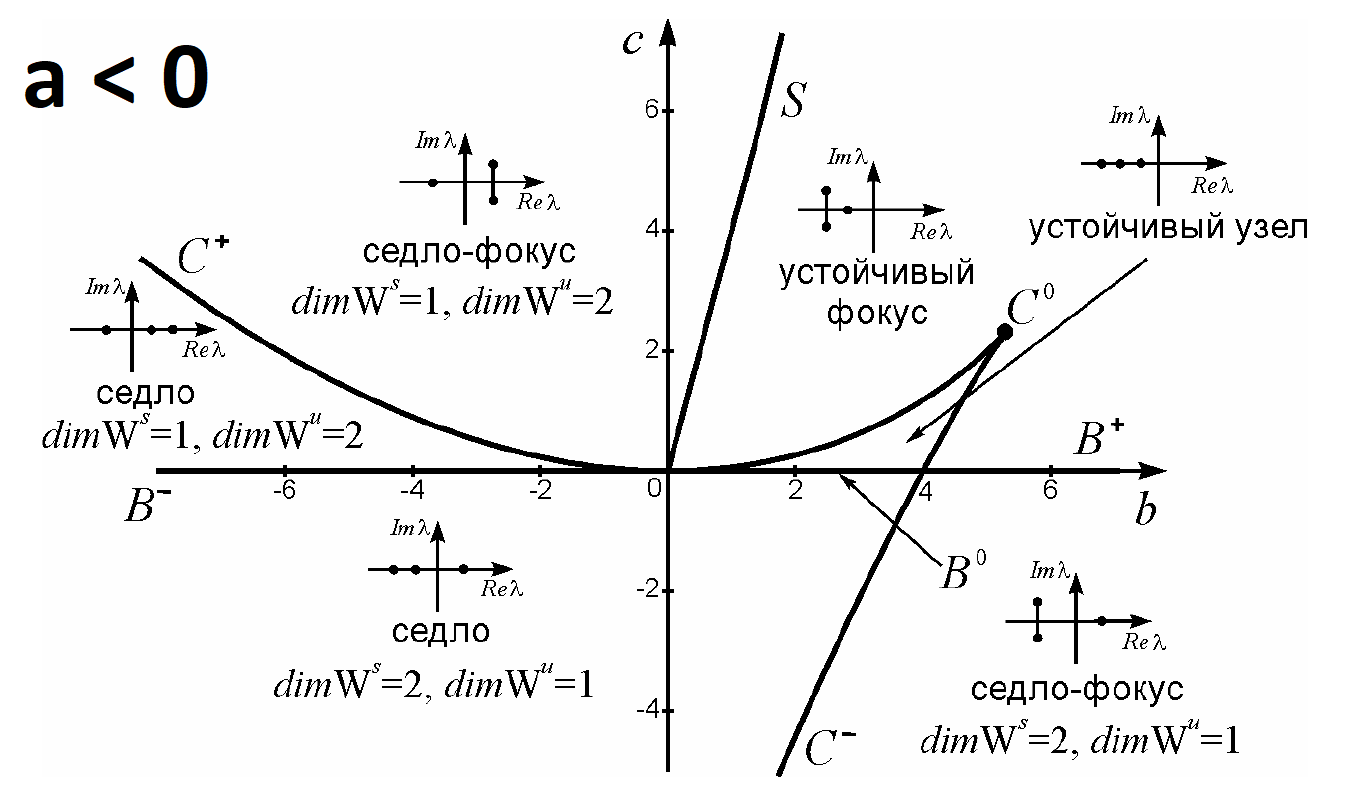
\includegraphics[width=0.5\linewidth]{tk_practice_img/classific_1}\\
		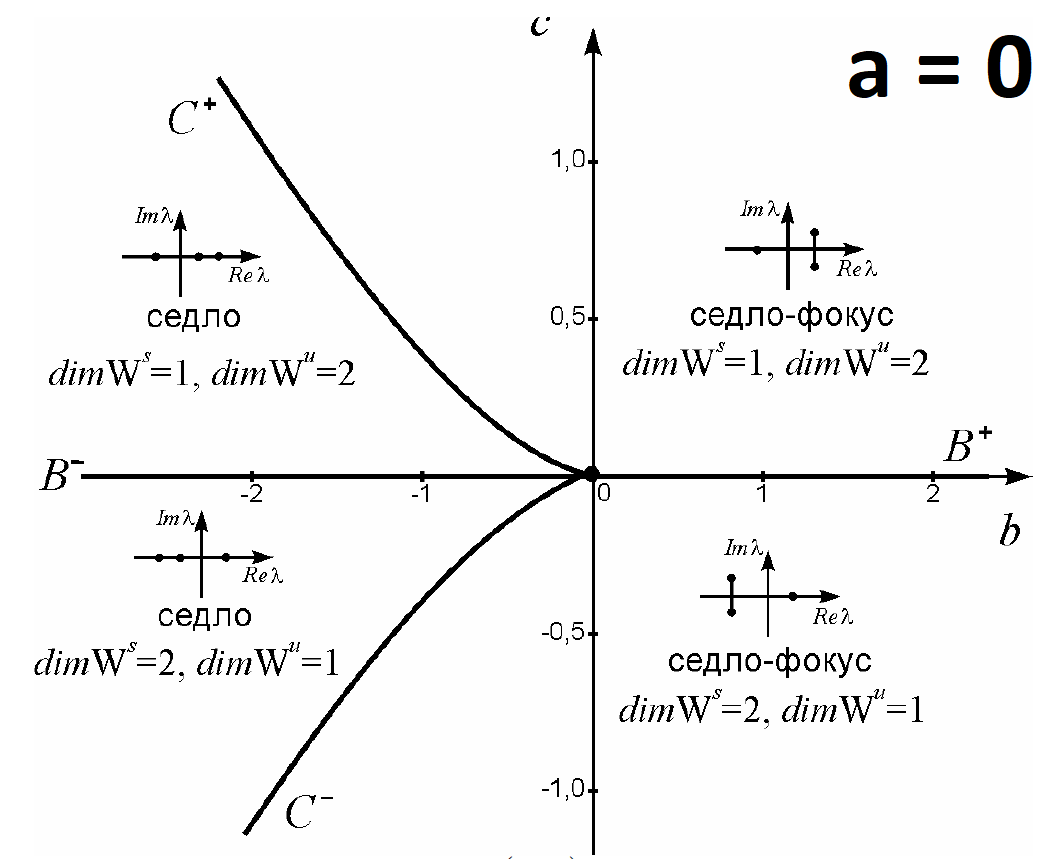
\includegraphics[width=0.5\linewidth]{tk_practice_img/classific_2}
		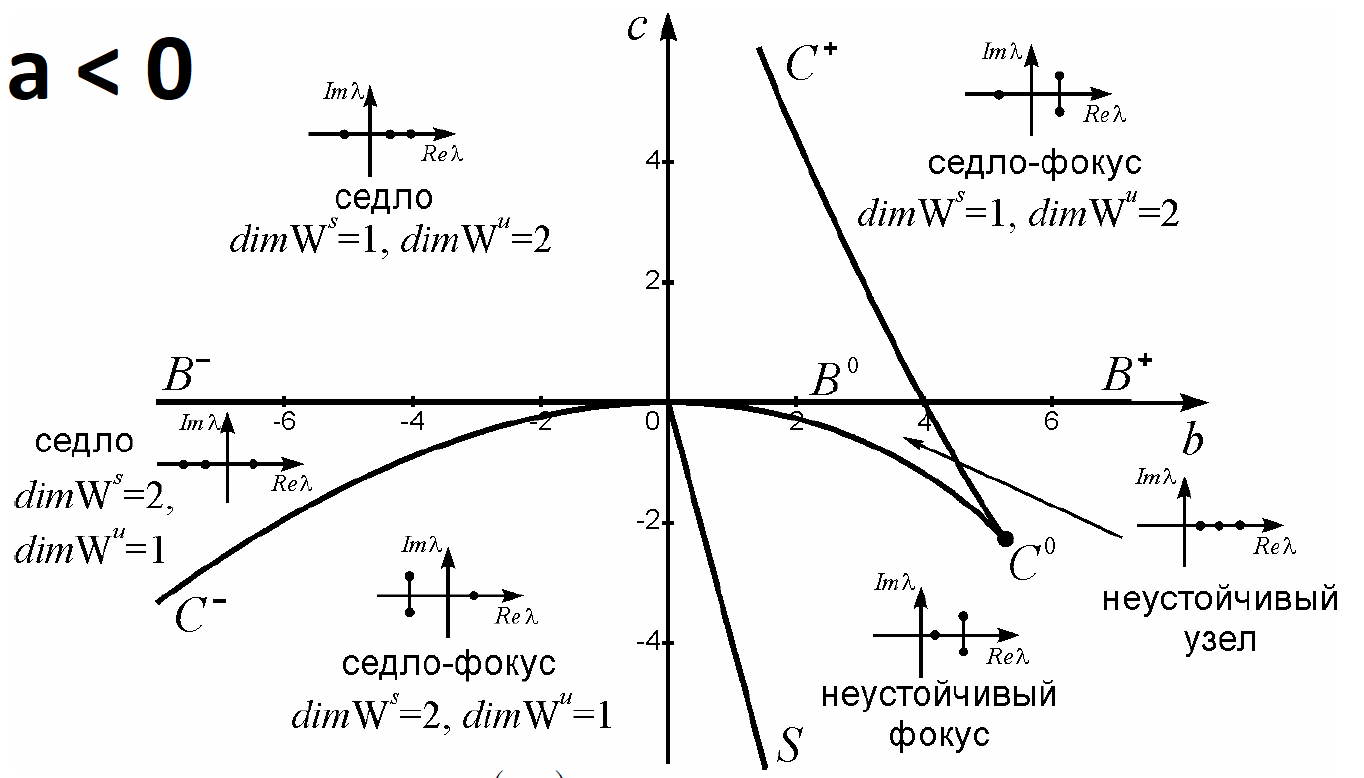
\includegraphics[width=0.5\linewidth]{tk_practice_img/classific_3}\\

	\end{multicols*}
\end{document}